\documentclass{article}
\usepackage{xeCJK}
% if you need to pass options to natbib, use, e.g.:
%\PassOptionsToPackage{numbers, compress}{natbib}
% before loading nips_2017
%
% to avoid loading the natbib package, add option nonatbib:
% \usepackage[nonatbib]{nips_2017}

\usepackage[final]{nips_2017}

% to compile a camera-ready version, add the [final] option, e.g.:
% \usepackage[final]{nips_2017}

\usepackage[utf8]{inputenc} % allow utf-8 input
\usepackage[T1]{fontenc}    % use 8-bit T1 fonts
\usepackage{hyperref}       % hyperlinks
\usepackage{url}            % simple URL typesetting
\usepackage{booktabs}       % professional-quality tables
\usepackage{amsfonts}       % blackboard math symbols
\usepackage{nicefrac}       % compact symbols for 1/2, etc.
\usepackage{microtype}      % microtypography
\usepackage{bm}             % bold in math
\usepackage{graphicx}       % images
\usepackage{algorithm}      % algorithm
\usepackage[noend]{algpseudocode} % algorithm
\usepackage{caption}        % captionof
\usepackage{array}          % thick column hline
\usepackage{booktabs}       % table style
\usepackage{pbox}           % table line break
\usepackage{subcaption}     % multiple figures
\usepackage{listings}
\usepackage{xcolor}
\usepackage{tikz}
\usepackage{amsmath}
\definecolor{mygreen}{rgb}{0,0.6,0}
\definecolor{mygray}{rgb}{0.5,0.5,0.5}
\definecolor{mymauve}{rgb}{0.58,0,0.82}
\definecolor{codeBkg}{rgb}{0.85,0.85,0.85}

\lstset{ 
	backgroundcolor=\color{codeBkg},   % choose the background color; you must add \usepackage{color} or \usepackage{xcolor}; should come as last argument
	basicstyle=\footnotesize,        % the size of the fonts that are used for the code
	breakatwhitespace=false,         % sets if automatic breaks should only happen at whitespace
	breaklines=true,                 % sets automatic line breaking
	captionpos=b,                    % sets the caption-position to bottom
	commentstyle=\color{mygreen},    % comment style
	deletekeywords={...},            % if you want to delete keywords from the given language
	escapeinside={\%*}{*)},          % if you want to add LaTeX within your code
	extendedchars=true,              % lets you use non-ASCII characters; for 8-bits encodings only, does not work with UTF-8
	frame=no,	                   % adds a frame around the code
	keepspaces=true,                 % keeps spaces in text, useful for keeping indentation of code (possibly needs columns=flexible)
	keywordstyle=\color{blue},       % keyword style
	language=Octave,                 % the language of the code
	morekeywords={*,...},            % if you want to add more keywords to the set
	numbers=left,                    % where to put the line-numbers; possible values are (none, left, right)
	numbersep=5pt,                   % how far the line-numbers are from the code
	numberstyle=\tiny\color{mygray}, % the style that is used for the line-numbers
	rulecolor=\color{black},         % if not set, the frame-color may be changed on line-breaks within not-black text (e.g. comments (green here))
	showspaces=false,                % show spaces everywhere adding particular underscores; it overrides 'showstringspaces'
	showstringspaces=false,          % underline spaces within strings only
	showtabs=false,                  % show tabs within strings adding particular underscores
	stepnumber=1,                    % the step between two line-numbers. If it's 1, each line will be numbered
	stringstyle=\color{mymauve},     % string literal style
	tabsize=4,	                   % sets default tabsize to 2 spaces
	title=\lstname                   % show the filename of files included with \lstinputlisting; also try caption instead of title
}

\title{高级量化交易技术}

\hypersetup{
    colorlinks = true,
}
\makeatletter
\def\BState{\State\hskip-\ALG@thistlm}
\makeatother
\floatname{algorithm}{Procedure}
\renewcommand{\algorithmicrequire}{\textbf{Input:}}
\renewcommand{\algorithmicensure}{\textbf{Output:}}

\newcolumntype{?}{!{\vrule width 3pt}}

\author{
  闫涛 \\
  %% examples of more authors
  %% \And
  %% Nicholas Frosst \\
  %% Affiliation \\
  %% Address \\
  %% \texttt{email} \\
  %% \AND
  %% Geoffrey E. Hinton \\
  科技有限公司\\
  北京 \\
  \texttt{\{yt7589\}@qq.com} \\
  %% Affiliation \\
  %% Address \\
  %% \texttt{email} \\
  %% \And
  %% Coauthor \\
  %% Affiliation \\
  %% Address \\
  %% \texttt{email} \\
  %% \And
  %% Coauthor \\
  %% Affiliation \\
  %% Address \\
  %% \texttt{email} \\
}
\date{March 2018}

% \usepackage{natbib}
% \usepackage{graphicx}

\begin{document}






\maketitle
\begin{center}
\Large \textbf{第1章} \quad \textbf{时间序列基本特性}
\end{center}
\begin{abstract}
在本章中我们将讨论时间序列的基本特性,包括自相关性和平稳性。
\end{abstract}
\section{时间序列基本特性}
时间序列的自相关性是指时间序列过去与未来存在某种关系,是我们时间序列预测的基础。主要用自协方差函数(Autocovariance Function, AF)、自相关系数函数(Autocorrelation Coefficent Function, ACF)和偏自相关系数函数(Partial Autocorrelation Coefficient Function, PACF)来描述。
\subsection{随机变量统计量}
随机变量X其取值为$x$的均值定义为:
\begin{equation}
E(x) = \mu
\label{e000001}
\end{equation}
方差定义为:
\begin{equation}
\sigma ^{2} (x) = E\bigg[ \big( x - \mu \big)^{2} \bigg]
\label{e000002}
\end{equation}
其中$\sigma (x)$为标准差。
对于两个随机变量$x$和$y$,其协方差可以定义为:
\begin{equation}
\sigma (x, y) = E\bigg[ \big( x - \mu _{x} \big) \big( y - \mu _{y} \big) \bigg]
\label{e000003}
\end{equation}
在实际应用中,我们不可能知道真实的均值,只能使用统计量,因此协方差可以定义为:
\begin{equation}
Cov(x, y) = \frac{1}{n-1} \sum_{i=1}^{n} (x_{i} - \bar{x})(y_{i} - \bar{y})
\label{e000004}
\end{equation}
随机变量$x$和$y$的相关系数定义为:
\begin{equation}
\rho(x,y)=\frac{E[(x-\mu_{x})(y-\mu_{y})]}{\sigma _{x} \sigma _{y}}=\frac{\sigma(x,y)}{\sigma _{x} \sigma _{y}}
\label{e000005}
\end{equation}
采用统计量的表示方法为:
\begin{equation}
Cor(x,y)=\frac{Cov(x,y)}{std(x) \times std(y)}
\label{e000006}
\end{equation}
以上我们讨论的都是不同随机变量之间的关系,对于时间序列来说,我们可以把从不同时间点开始的子时间序列,视为不同的随机变量,那么我们就可以定义自协方差、自相关系数函数和偏自相关系数函数了。\newline
\subsection{时序序列平稳性}
时序信号$x_{t}$的均值定义为:
\begin{equation}
E(x_{t})=\mu (t)
\label{e000007}
\end{equation}
时间序列的均值与所考虑的时间点有关。我们可以把时间序列上每个时间点都视为一个独立的时间变量,但是对于时间序列而言,每个时间点的随机变量只有一个观测值,怎么求出均值呢?在实际应用中,我们会将时间序列中的趋势信号(上涨或下跌)、季节性信号等从时间序列中去除掉,对于剩下的残差序列,我们可以视为其各个时间点上的随机变量的均值是不变的,于是就可以使用下面的公式来计算均值:
\begin{equation}
\bar{x}=\frac{1}{N} \sum_{t=1}^{N}x_{t}
\label{e000008}
\end{equation}
由此我们引入平稳时间序列的概念,对于平稳时间序列,其各个时间点上对应的随机变量的均值相等。
时间序列的方差可以定义为:
\begin{equation}
\sigma ^{2}(t)=E[(x_{t}-\mu _t)^{2}]
\label{e000009}
\end{equation}
根据上面平稳时间序列的定义,各个时间点对应的随机变量的均值不变,则式\ref{e000009}可以化间为:
\begin{equation}
\sigma ^{2}(t)=E[(x_{t}-\mu)^{2}]
\label{e000010}
\end{equation}
我们同时规定,平稳时间序列各个时间点对应的随机变量的方差也不变,则\ref{e000010}可进一步化简为:
\begin{equation}
Var(x_{t})=\frac{1}{N-1} \sum_{t=1}{N} (x_t - \bar{x})^{2}
\label{e000011}
\end{equation}
\subsection{自协方差}
在讨论自协方差之前,我们首先要定义二阶平稳性。根据上一节定义,平稳时间序列是指各个时间点对应的随机变量的均值和方差相同。二阶平稳性是指在这一基础上,不同时间点对应的随机变量的相关系数只与时间相隔(lag)相关。注意:以下我们讨论的各种性质,均以此为前提。
对于lag=k的自协方差定义为:
\begin{equation}
C_{k}=E[(x_{t} - \mu)(x_{t+k} - \mu)]
\label{e000012}
\end{equation}
\subsection{自相关系数函数ACF}
由于自协方差的大小与随机变量的大小有关,无法准确衡量其间的关系,因此我们引入自相关系数函数ACF:
\begin{equation}
\rho _{k} = \frac{C_{k}}{\sigma ^{2}}
\label{e000013}
\end{equation}
由定义可知:
\begin{equation}
\begin{aligned}
\rho _{0} = \frac{C_{0}}{\sigma ^{2}} = \frac{E[(x_{t} - \mu)(x_{t} - \mu)]}{\sigma ^{2}} \\
= \frac{E[(x_{t} - \mu)^{2}]}{\sigma ^{2}} = \frac{\sigma ^{2}}{\sigma ^{2}} = 1\\
\end{aligned}
\label{e000014}
\end{equation}
在实际应用中,我们都是处理的离散数据点,则自协方差可以定义为:
\begin{equation}
c_{k}=\frac{1}{N}\sum_{t=1}^{N}(x_{t}-\bar{x})(x_{t+k} - \bar{x})
\label{e000015}
\end{equation}
自相关系数函数ACF可以定义为:
\begin{equation}
r_{k}=\frac{c_{k}}{c_{0}}
\label{e000016}
\end{equation}
\subsection{自相关性举例}
下面我们以上证综指时间序列为例,来看自相关系数函数ACF和偏自相关系数函数PACF的求法和作图,程序代码如下所示:
\lstset{language=PYTHON, caption={时间序列基本性质}, label={c000001}}
\begin{lstlisting}
import pandas as pd
import matplotlib.pyplot as plt
import matplotlib.dates as mdates
from matplotlib.font_manager import FontProperties
from statsmodels.tsa import stattools
from statsmodels.graphics import tsaplots

class Chp023(object):
    def __init__(self):
        self.name = 'Chp022'
        # 数据文件格式:编号 日期 星期几 开盘价 最高价 
        # 最低价 收益价 收益
        self.data_file = 'data/pqb/chp023_001.txt'
        
    def startup(self):
        print('第23章:时间序列基本性质')
        data = pd.read_csv(self.data_file, sep='\t', index_col='Trddt')
        sh_index = data[data.Indexcd==1]
        sh_index.index = pd.to_datetime(sh_index.index)
        sh_return = sh_index.Retindex
        print('时间序列长为:N={0}'.format(len(sh_return)))
        acfs = stattools.acf(sh_return)
        print(acfs)
        pacfs = stattools.pacf(sh_return)
        print(pacfs)
        tsaplots.plot_acf(sh_return, use_vlines=True, lags=30)
        plt.show()
        tsaplots.plot_pacf(sh_return, use_vlines=True, lags=30)
        plt.show()
\end{lstlisting}
数据文件格式为:
\begin{figure}[H]
	\caption{数据文件格式}
	\label{f000001}
	\centering
	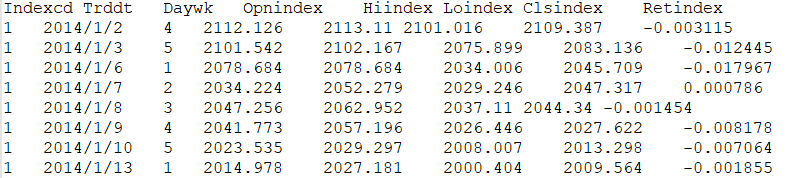
\includegraphics[height=3cm]{images/f000001}
\end{figure}
其运行结果为:
\begin{figure}[H]
	\caption{运行结果}
	\label{f000002}
	\centering
	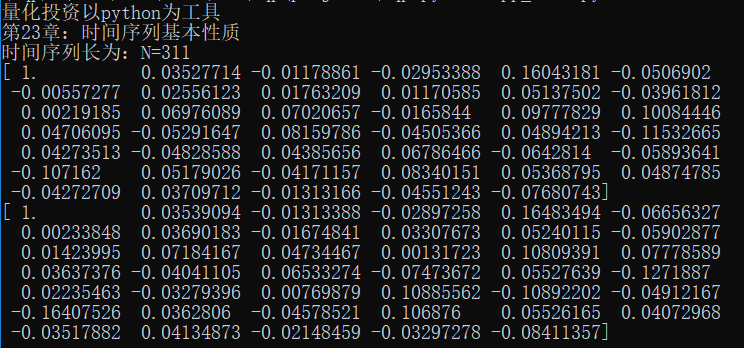
\includegraphics[height=3cm]{images/f000002}
\end{figure}
在图\ref{f000002}中,第一个数据为自相关系数函数ACF各期的值,而第二个数组为偏自相关系数函数PACF各期的值。判断时间序列是否具有自相关性,可以看除ACF和PACF中,除第一个元素外,有没有显著超过阈值的元素,阈值定义为:
\begin{equation}
threshold=\frac{1.96}{\sqrt{N}} = \frac{1.96}{\sqrt{311}} = 0.11
\label{e000017}
\end{equation}
式\ref{e000017}中的N为时间序列样本数,在本例中,共有311条记录,故N=311,所以其阈值为0.11左右。由于$acf[4]=0.16>0.11$所以可以推断其具有自相关性,同时$pacf[4]=0.165>0.11$也可以推断其具有自相关性。我们还可以通过图形的方式形像的表示出来,自相关系数函数图如所示:
\begin{figure}[H]
	\caption{自相关系数函数图}
	\label{f000003}
	\centering
	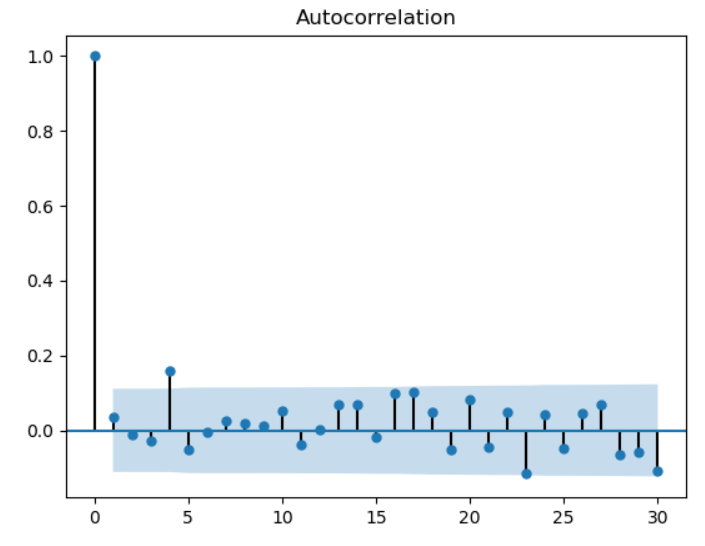
\includegraphics[height=4cm]{images/f000003}
\end{figure}
图\ref{f000003}中蓝色区域的界限为$[-\frac{1.96}{\sqrt{N}}, \frac{1.96}{\sqrt{N}}]=[-0.11, 0.11]$,除第1项外,其他项如果超出蓝色区域则说明此时间序列具有自相关性。\newline
偏自相关系数函数图为:
\begin{figure}[H]
	\caption{偏自相关系数函数图}
	\label{f000004}
	\centering
	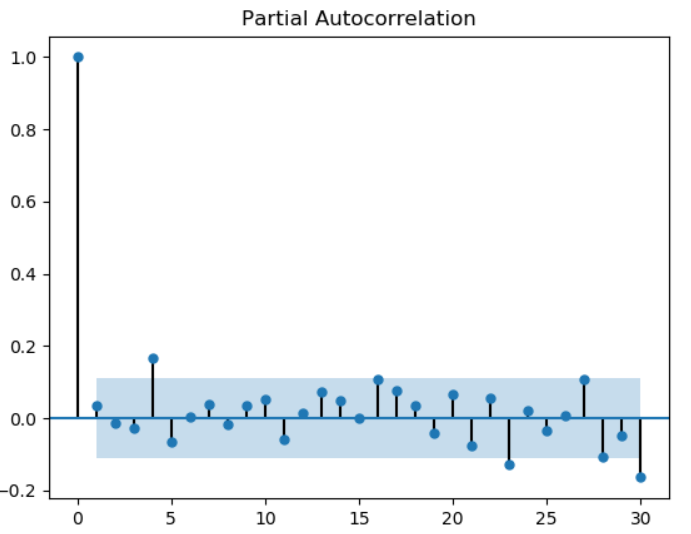
\includegraphics[height=4cm]{images/f000004}
\end{figure}
\subsection{白噪声和随机游走}
\subsubsection{残差序列定义}
我们要对任意时间序列$y_{t}$进行建模,我们的模型为$\hat{y}_{t}$,残差序列$x_{t}$可以定义为:$x_{t}=y_{t}-\hat{y}_{t}$,我们的任务就是使残差时间序列中每一个时间点对应的随机变量互相独立,没有自相关性,即满足独立同分布(Independent and Identical Distribution,I.I.D)条件。如果各个随机变量$x_{t} \sim \mathbb{N}(0, \sigma ^{2})$,则称其为高斯白噪声。\newline
\subsubsection{差分运算符}
为了后续讨论问题方便,我们首先定义BSO运算符:
\begin{equation}
Bx_{t}=x_{t-1} \quad B^{n}x_{t}=x_{t-n}
\label{e000018}
\end{equation}
我们定义差分运算符为:
\begin{equation}
\begin{aligned}
\nabla x_{t} = x_{t}-x_{t-1}=(1-B)x_{t} \\
\nabla x_{t}^{n} = \big( x_{t}-x_{t-n} \big)^{n}=(1-B)^{n}x_{t}
\end{aligned}
\label{e000019}
\end{equation}
\subsubsection{白噪声定义}
对于时间序列$\{ w_{t}, t=1,2,3,...,N \}$,满足$\forall t \quad w_{t} \sim \mathcal{N}(0, \sigma ^{2})$且$\forall i \ne j \quad Cor(w_{i}, w_{j})=0$,则其为白噪声时间序列。\newline
下面我们来看白噪声的二阶属性:
\begin{equation}
\begin{aligned}
\mu = E(w_{t})=0 \\
\gamma _{k}= Cor(w_{t}, w_{t+k}) = \begin{cases}
1 \quad if \quad k=0 \\
0 \quad if \quad k \ne 0
\end{cases}
\end{aligned}
\label{e000020}
\end{equation}
\subsubsection{随机游走}
随机游走(Random Walk)时间序列是指$x_{t}$可以定义为:$x_{t}=x_{t-1}+w_{t}$,其中$w_{t}$为白噪声时间序列。随机游走时间序列可以表示为:
\begin{equation}
\begin{aligned}
x_{t}=x_{t-1}+w_{t}=Bx_{t}+w_{t} \\
x_{t}=x_{t-1}+w_{t}=x_{t-2}+w_{t-1}+w_{t} \\
...... \\
x_{t}=w_{1} + w_{2} + ... + w_{t-1} + w_{t}
\end{aligned}
\label{e000021}
\end{equation}
所以随机游走时间序列可以看作是多个白噪声时间序列的叠加。下面我们来看随机游走时间序列的均值和协方差:
\begin{equation}
\begin{aligned}
\mu = 0 \\
\gamma _{k}(t)=Cov(x_{t}, x_{t+k})=t \sigma ^{2}
\end{aligned}
\label{e000022}
\end{equation}
我们再来看随机游走序列的自相关系数函数ACF:
\begin{equation}
\begin{aligned}
\rho _{k}(t)=\frac{Cov(x_{t}, x_{t+k})}{\sqrt{ Var(x_{t}) \cdot Var(x_{t+k}) }} \\
=\frac{t \sigma ^{2}}{\sqrt{t \sigma ^{2} (t+k) \sigma ^{2}}}=\frac{1}{\sqrt{1+ \frac{k}{t} }}
\end{aligned}
\label{e000023}
\end{equation}
在通常情况下,t比k要大得多,因此$\rho_{k}$会比较接近于1。\newline
下面我们来模拟一个随机游走时间序列信号,程序如下所示:
\lstset{language=PYTHON, caption={随机游走过程模拟}, label={c000003}}
\begin{lstlisting}
    def random_wale_demo(self):
        '''
        随机游走时间序列建模示例
        '''
        w = np.random.standard_normal(size=1000)
        x = w
        for t in range(1, len(w)):
            x[t] = x[t-1] + w[t]
        plt.plot(x, c='b')
        plt.title('Random Walk Demo')
        plt.show()
        acfs = stattools.acf(x)
        print(acfs)
        tsaplots.plot_acf(x, use_vlines=True, lags=30)
        plt.show()
        # 拟合随机游走信号
        r = []
        for t in range(1, len(x)):
            r.append(x[t] - x[t-1])
        rd = np.array(r)
        plt.plot(rd, c='r')
        plt.title('Residue Signal')
        plt.show()
        rd_acfs = stattools.acf(rd)
        print(rd_acfs)
        tsaplots.plot_acf(rd, use_vlines=True, lags=30)
        plt.show()
\end{lstlisting}
我们首先通过$x_{t}=x_{t-1}+w_{t}$生成一个随机游走信号,该信号图形如下所示:
\begin{figure}[H]
	\caption{随机游走时间序列信号}
	\label{f000005}
	\centering
	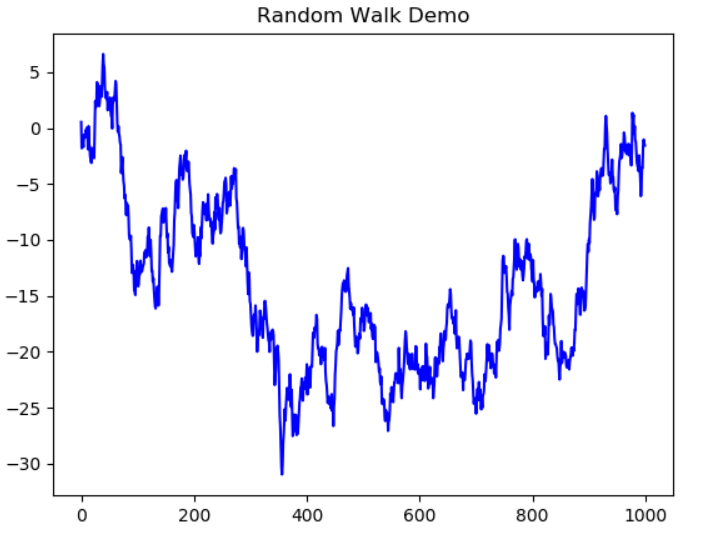
\includegraphics[height=5cm]{images/f000005}
\end{figure}
由图\ref{f000005}可以看出,其非常像是一个股票收盘价的走势图,这也是为什么有些人说股票走势是随机游走过程了。接着我们求出该时间序列的自相关系数函数ACF及其自相关图,如下所示:
\begin{figure}[H]
	\caption{随机游走时间序列信号}
	\label{f000006}
	\centering
	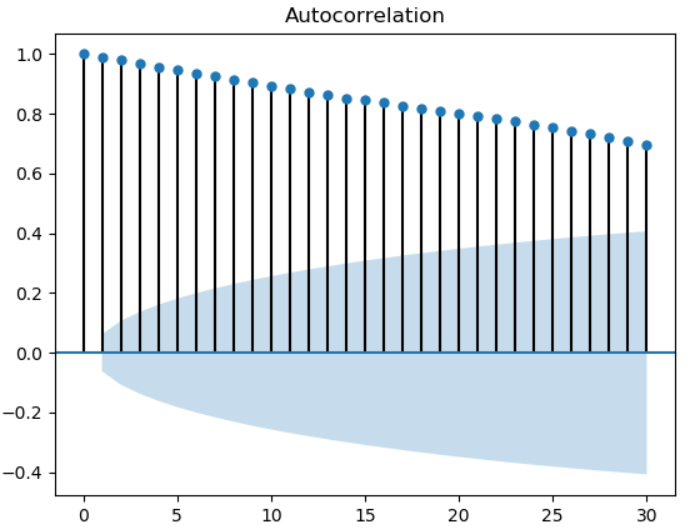
\includegraphics[height=5cm]{images/f000006}
\end{figure}
由图可以看出,其具有极强的自相关性,所有ACF值均位于蓝色置信区间之外。\newline
我们知道$x_{t}-x_{t-1}=w_t$,而$w_t$是白噪声时间序列信号,这实际上模拟了实际应用过程,我们把$x_t$视为实际的金融信号,而$x_{t-1}$为我们建模的信号,将两个信号相减,得到残差信号,如果残差信号是白噪声信号,就可以认为我们建模是合理的。下面来看我们得到的残差信号:
\begin{figure}[H]
	\caption{残差时间序列信号}
	\label{f000007}
	\centering
	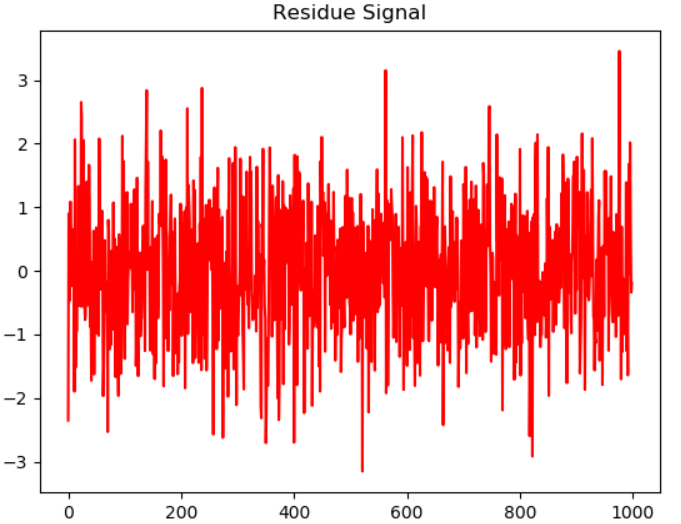
\includegraphics[height=5cm]{images/f000007}
\end{figure}
计算并绘制ACF如下所示:
\begin{figure}[H]
	\caption{残差自相关系数函数}
	\label{f000008}
	\centering
	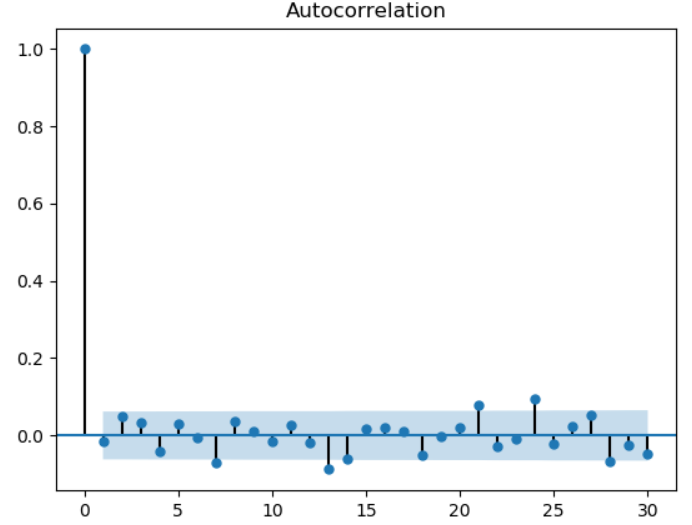
\includegraphics[height=5cm]{images/f000008}
\end{figure}
程序的运行结果如下所示:
\begin{figure}[H]
	\caption{程序运行结果}
	\label{f000009}
	\centering
	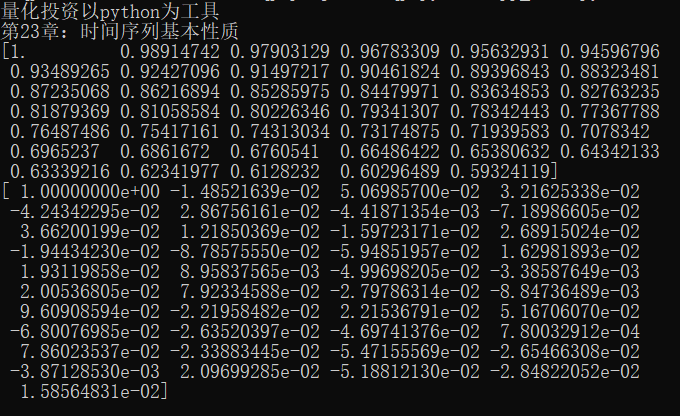
\includegraphics[height=5cm]{images/f000009}
\end{figure}
下面我们以上证综指收益率为例,来看随机游走模型是否可以很好的拟合这个时间序列,程序如下所示:
\lstset{language=PYTHON, caption={随机游走拟合上证综指收益率}, label={c000004}}
\begin{lstlisting}
    def random_walk_fit(self):
        data = pd.read_csv(self.data_file, sep='\t', index_col='Trddt')
        sh_index = data[data.Indexcd==1]
        sh_index.index = pd.to_datetime(sh_index.index)
        sh_return = sh_index.Retindex
        print('时间序列长为:N={0}'.format(len(sh_return)))
        r = []
        for t in range(1, len(sh_return)):
            r.append(sh_return[t] - sh_return[t-1])
        rd = np.array(r)
        plt.plot(rd, c='b')
        plt.title('Random Walk fit SHIndex Return')
        plt.show()
        rd_acfs = stattools.acf(rd)
        print(rd_acfs)
        tsaplots.plot_acf(rd, use_vlines=True, lags=30)
        plt.show()
\end{lstlisting}
其残差图像为:
\begin{figure}[H]
	\caption{残差图形}
	\label{f000010}
	\centering
	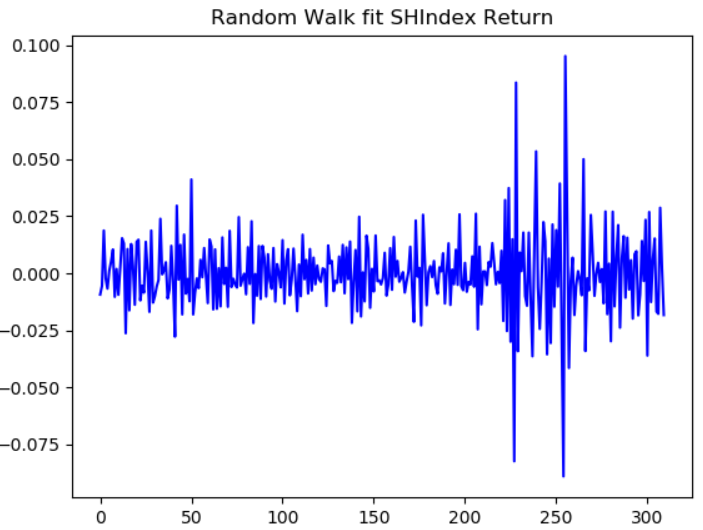
\includegraphics[height=5cm]{images/f000010}
\end{figure}
自相关系数函数ACF图形:
\begin{figure}[H]
	\caption{自相关系数函数ACF}
	\label{f000011}
	\centering
	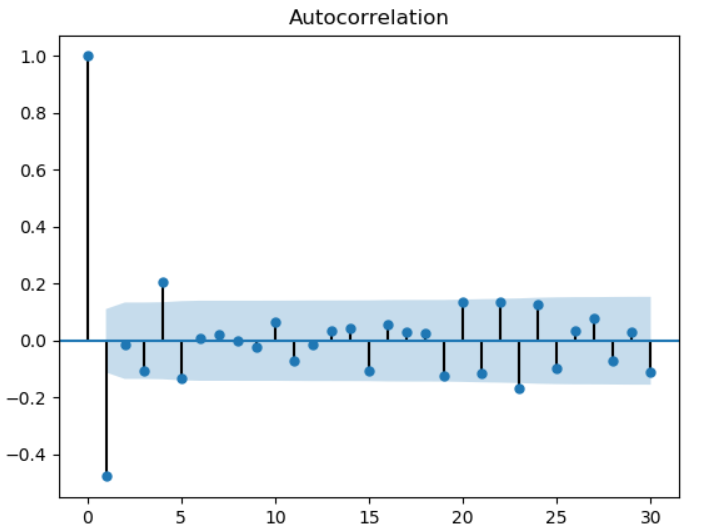
\includegraphics[height=5cm]{images/f000011}
\end{figure}
由图\ref{f000011}所示,在1、4时间点,明显超出置信范围,因此随机游走过程不能很好的拟合上证综指收益率时间序列信号。程序的运行结果如下所示:
\begin{figure}[H]
	\caption{程序运行结果}
	\label{f000012}
	\centering
	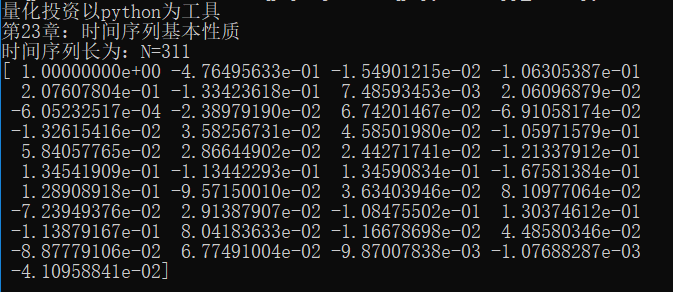
\includegraphics[height=5cm]{images/f000012}
\end{figure}

\maketitle\begin{center}
\Large \textbf{第2章 ARIMA模型}
\end{center}
\begin{abstract}
在本章中我们将首先讲述自回归模型AR(p),接着讲述移动平均MA(q),最后讲解ARMA(p,q),然后将其泛化为ARIMA(p,d,q),
分别将这些模型用于实际金融时间序列数据拟合。aqt001.py
\end{abstract}
\section{ARIMA模型}
\subsection{稳定性和模型选择标准}
\subsubsection{强稳定性}
在我们以前的讨论中,我们说如果一个时间序列各个时间点所对应的随机变量,只要均值和方差不变,就是平稳时间序列。下面我们对强平稳性进行定义。\newline
对于一个时间序列$\{ x_{t} \}$,如果对于$\forall t_{i},m$,两个序列:$x_{t_1}, x_{t_2},...,x_{t_N}$和$x_{t_1+m}, x_{t_2+m},...,x_{t_N+m}$的统计特性完全相同,则说明该时间序列为强平稳特性。
\subsubsection{模型选择标准}
我们将用AIC来进行模型选择,AIC的全称为:Akaike Information Criterion,我们通常会选择AIC值较小的模型。在实际应用中,还可以使用BIC来进行模型选择,BIC的全称为Bayes Information Criterion。在本章中我们只用AIC来进行模型选择。\newline
假设统计模型的似然函数有$k$参数,最大似然值为$L$,则AIC定义为:
\begin{equation}
AIC=-2\log(L) + 2k
\label{e000024}
\end{equation}
由式\ref{e000024}可知,最大似然值越大或者参数越少,AIC的值越小,模型就越是好模型。
\subsubsection{ADF检验}
在前面所讨论的问题中,我们通常根据自相关系数函数ACF和偏自相关系数函数PACF来判断稳定性,但是主观性比较强,我们需要一个客观的标准。\newline
我们首先来定义时间序列的阶数,对于下面的非平稳时间序列:
\begin{equation}
x_{t}=x_{t-1}+w_{t}
\label{e000036}
\end{equation}
其中$w_{t} \sim \mathcal{N}(0, \sigma ^{2})$为白噪声信号,且$x_{0}=0$,我们可以得到其均值为:
\begin{equation}
E(x_{t})=E(x_{t-1}+w_{t})=E(x_{t-1})+E(w_{t})=E(x_{t-1})=...=E(x_{0})=0
\label{e000037}
\end{equation}
同样我们可以得到其方差:
\begin{equation}
Var(x_{t})=Var(x_{t-1}+w_{t})=Var(x_{t-1})+Var(w_{t})=Var(x_{t-1})+\sigma ^{2}=...=t\sigma ^{2}
\label{e000038}
\end{equation}
$x_{t}$由于其各时间点对应的随机变量的方差随时间变化,因此不是平稳时间序列。\newline
我们定义1阶差分算子:
\begin{equation}
\nabla x_{t} = Bx_{t}=x_{t}-x_{t-1}=w_{t}
\label{e000039}
\end{equation}
对于$Bx_{t}$为白噪声信号,其显然是平稳时间序列,所以我们称$x_{t}$为I(1)的非平稳时间序列。我们可以将其定义扩展到$n$阶:
\begin{equation}
Bx_{t}=x_{t-1} \quad B^{2}x_{t}=x_{t-2} \quad B^{3}x_{t}=x_{t-3} \quad ...  \quad B^{n}x_{t}=x_{t-n}
\label{e000040}
\end{equation}
我们还以上面的时间序列$x_{t}=x_{t-1}+w_t$为例,我们可以将其写为:
\begin{equation}
x_{t}-x_{t-1}=x_{t}-Bx_{t}=(1-B)x_{t}=w_{t}
\label{e000041}
\end{equation}
式\ref{e000041}中$1-B$为滞后算子多项式,我们令$1-B=0$得出的解为$B=1$,其为单位根,所以其为非平稳时间序列。这一结论可以推广到更一般的情况,对于如下所示的时间序列:
\begin{equation}
y_{t}=(1+\rho)y_{t-1}-\rho y_{t-2}+w_{t}
\label{e000042}
\end{equation}
其所对应的滞后算子多项式为:
\begin{equation}
y_{t}-(1-\rho)By_{t}+\rho B^{2} y_{t}=w_{t}
\label{e000043}
\end{equation}
令式\ref{e000043}左边为0,得到的解为:$B=1$和$B=\frac{1}{\rho}$,因为其存在单位根,所以其不是平稳时间序列。\newline
对于任意如下所示时间序列:
\begin{equation}
y_{t}=\gamma + \rho _{1}y_{t-1} + \rho _{2}y_{t-2} + ... + \rho _{p}y_{t-p} + w_{t}
\label{e000044}
\end{equation}
其中$w_{t} \sim \mathcal{N}(0, \sigma ^{2})$为独立同分布(i.i.d)噪声信号。
可以将式\ref{e000044}改写为如下形式:
\begin{equation}
y_{t}=\gamma + \rho _{1}By_{t} + \rho _{2}B^{2}y_{t} + ...  + \rho _{p}B^{p}y_{t} + w_{t}
\label{e000045}
\end{equation}
将式\ref{e000045}右边所有包含$y_{t}$的项都移到左边,可以得到下式:
\begin{equation}
(1-\rho _{1}B - \rho _{2}B^{2} - .. - \rho _{p}B^{p})y_{t}=\gamma + w_{t}
\label{e000046}
\end{equation}
可以得到其对应的滞后算子多项式方程为:
\begin{equation}
1-\rho(B)=1-\rho _{1}B - \rho _{2}B^{2} - .. - \rho _{p}B^{p}=0
\label{e000047}
\end{equation}
解这个方程,如果所有解的绝对值均大于1,则该时间序列为平稳时间序列,如果存在单位根或绝对值小于1的根,则其为非平稳时间序列。\newline
以上我们讲解的判断时间序列平稳性的原理,在实际应用中,我们通常采用ADF来判断时间序列的平稳性,ADF模型如下所示:
\begin{equation}
\Delta y_{t}=\alpha + \beta t + \gamma y_{t-1} + \delta _{1}\Delta y_{t-1} + \delta _{2}\Delta y_{t-2} + ... + \delta _{p}\Delta y_{t-p} + w_{t}
\label{e000048}
\end{equation}
其中$\alpha$对应截距,$\beta$对应趋势,$\delta _{1}\Delta y_{t-1} + \delta _{2}\Delta y_{t-2} + ... + \delta _{p}\Delta y_{t-p}$为ADF的增广项,p为增广项的期数,其值由AIC或BIC算法来决定。原假设$H_{0}$为该序列有单位根是非平稳时间序列:$\gamma = 0$;备择假设$H_{1}$为该序列为平稳时间序列:$\gamma < 0$。\newline
这部分原理比较复杂,我们在实际应用中,通常使用arch包中的ADF函数来完成检验工作,其函数定义为:
\begin{equation}
ADF(y, lags, trend, max_lags, method)
\label{e000049}
\end{equation}
其中:
\begin{itemize}
\item y:待判断的时间序列;
\item lags:滞后期数
\item trend:用来控制检验模型的类型
	\begin{itemize}
	\item 'nc':不含截距项;
	\item 'c':含截距项;
	\item 'ct':包含截距项和线性趋势项;
	\item 'ctt':包含截距项和线性趋势项以及二次趋势项;
	\end{itemize}
\item max\_lags:最大期数
\item method:常用方法为:'aic'、 'bic'、 't\_stat'
\end{itemize}
下面我们通过一个例子来看怎样使用ADF方法,我们以上证综指收益率和收盘价这两个序列为例,我们首先需要安装python的garch库:
\lstset{language=BASH}
\begin{lstlisting}
pip install arch
\end{lstlisting}
程序代码如下所示:
\lstset{language=PYTHON, caption={ADF检验}, label={c000006}}
\begin{lstlisting}
import arch.unitroot as unitroot
......
    def adf_demo(self):
        print('ADF检验例程...')
        data = pd.read_csv(self.data_file, sep='\t', index_col='Trddt')
        sh_index = data[data.Indexcd==1]
        sh_index.index = pd.to_datetime(sh_index.index)
        sh_return = sh_index.Retindex
        sh_return_adf = unitroot.ADF(sh_return)
        print(sh_return_adf.summary().as_text())
        print('stat={0:0.4f}; pvalue={0:0.4f}'.format(sh_return_adf.stat, sh_return_adf.pvalue))
        print('critical_values:{0}'.format(sh_return_adf.critical_values))
        print('1%value={0}'.format(sh_return_adf.critical_values['1%']))
        if sh_return_adf.stat < sh_return_adf.critical_values['1%']:
            print('上证综指收益率为平稳时间序列 ^_^')
        else:
            print('上证综指收益率为平稳时间序列  !!!!!!!!!')
        sh_close = sh_index.Clsindex
        sh_close_adf = unitroot.ADF(sh_close)
        if sh_close_adf.stat < sh_close_adf.critical_values['1%']:
            print('上证综指收盘价为平稳时间序列 ^_^')
        else:
            print('上证综指收盘价为非平稳时间序列 !!!!!!!')
\end{lstlisting}
运行结果如下所示:
\begin{figure}[H]
	\caption{自相关系数函数ACF}
	\label{f000022}
	\centering
	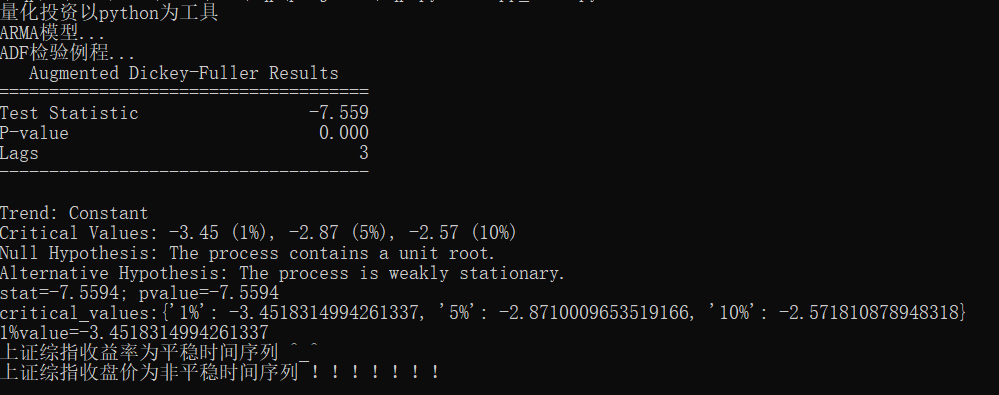
\includegraphics[height=5cm]{images/f000022}
\end{figure}
由上面的结果可以看出,上证综指收益率是稳定的时间序列,收盘价却是不稳定的时间序列。
\subsection{自回归模型}
\subsubsection{背景}
我们可以扩展随机游走模型,使当前时间点数据不仅依赖前一时间点的值,同时还依赖前p个时间点的值,是这p个值的线性组合,
这就得到了自回归模型。
\subsubsection{模型定义}
自回归模型AR(p)是随机游走模型的扩展,p阶自回归模型定义为:
\begin{equation}
x_{t}=\alpha _{1}x_{t-1} + \alpha _{2}x_{t-2} + ... + \alpha _{p}x_{t-p} + w_{t} = \sum_{i=1}^{p} \alpha _{i}x_{t-i} + w_{t}
\label{e000025}
\end{equation}
其中$\{ w_{t} \}$为白噪声,$\alpha _{i} \in R$且$\alpha_{p} \ne 0$。\newline
当$p=1$且$\alpha _{1}=1$时,自回归模型就退化为随机游走模型。\newline
为后续讨论方便,我们定义如下运算符:
\begin{equation}
\theta _{p}(B)x_{t}=(1-\alpha _{1}B-\alpha _{2}B^{2}-...-\alpha _{p}B^{p})x_{t}=w_{t}
\label{e000026}
\end{equation}
有了上述模型之后,我们就可以直接拿来作预测,如下所示:
\begin{equation}
\begin{aligned}
    \hat{x}_t=\alpha _{1}x_{t-1}+\alpha _{2}x_{t-2}+...+\alpha _{p}x_{t-p} \\
    \hat{x}_{t+1}=\alpha _{1}\hat{x}_{t}+\alpha _{2}x_{t-1}+...+\alpha _{p}x_{t-p+1}
\end{aligned}
\label{e000027}
\end{equation}
然后依此类推,可以求出其后n个时间点的预测值。
\subsubsection{二阶特性}
我们首先定义特性方程:
\begin{equation}
\theta _{p}(B)=0
\label{e000028}
\end{equation}
解这个方程得到的解的绝对值必须大于才是平稳序列。我们可以举几个实例,首先是随机游走序列:
\paragraph{随机游走}
根据定义$x_{t}=x_{t-1}+w_{t}$我们可以得到$\alpha _1=1$,其特性方程为$\theta=1-B=0$,其解为$B=1$,因为其解的
绝对值不大于1,所以其不是平稳模型。
\paragraph{1阶自回归}
我们假设自回归模型为$x_{t}=\frac{1}{4}x_{t-1}+w_{t}$,其中$\alpha _1=\frac{1}{4}$,
其特性方程为$\theta = 1-\frac{1}{4}=0$,其解为$B=4$,该解绝对值大于1,所以其是平稳模型。
\paragraph{2阶自回归模型}
我们假设自回归模型为$x_{t}=\frac{1}{2}x_{t-1}+\frac{1}{2}x_{t-2}+w_{t}$,其特性方程为
$\theta _2(B)=\frac{1}{2}(1-B)(B+2)=0$,则其解为$B=1,-2$,其中一个解为单位根,其绝对值不大于1,因此本模型不是
平稳模型。虽然本模型不是平稳模型,但是其他2阶自回归模型是完全有可能是平稳模型的。
\paragraph{二阶特性}
均值、自协方差、自相关系数定义如下所示:
\begin{equation}
\begin{aligned}
\mu _{x}=E(x_{t})=0 \\
\gamma _{k}=\sum_{i=1}^{p}\alpha _{i} \gamma _{k-i}, \quad k>0 \\
\rho _{k} = \sum_{i=1}^{p}\alpha _{i} \rho _{k-i}, \quad k>0
\end{aligned}
\label{e000029}
\end{equation}
\subsubsection{模拟数据}
下面我们来模拟一个AR(2)的时间序列,我们的数据生成和拟合代码如下所示:
\lstset{language=PYTHON, caption={AR数据模拟和拟合示例}, label={c000004}}
\begin{lstlisting}
import numpy as np
import pandas as pd
import matplotlib.pyplot as plt
import matplotlib.dates as mdates
from matplotlib.font_manager import FontProperties
from statsmodels.tsa import stattools
from statsmodels.graphics import tsaplots
from statsmodels.tsa.arima_model import ARIMA

class Aqt001(object):
    def __init__(self):
        self.name = 'Aqt001'
        
    def startup(self):
        print('ARMA模型...')
        self.simulate_ar2()
        
    def simulate_ar2(self):
        print('模拟AR(2)')
        alpha1 = 0.666
        alpha2 = -0.333
        wt = np.random.standard_normal(size=1000)
        x = wt
        for t in range(2, len(wt)):
            x[t] = alpha1 * x[t-1] + alpha2 * x[t-2] + wt[t]
        plt.plot(x, c='b')
        plt.show()
        ar2 = stattools.ARMA(x, (2, 0)).fit(disp=False)
        print('p={0} **** {1}; q={2}***{3}; {4} - {5} - {6}'.format(
                    ar2.k_ar, ar2.arparams, ar2.k_ma, ar2.maparams, 
                    ar2.aic, ar2.bic, ar2.hqic)
        )
        arima2_0_0 = ARIMA(x, order=(2, 0, 0)).fit(disp=False)
        print('ARIMA: p={0} **** {1}; q={2}***{3}; {4} - {5} - {6}'. \
                    format(arima2_0_0.k_ar, arima2_0_0.arparams, 
                    arima2_0_0.k_ma, arima2_0_0.maparams, 
                    arima2_0_0.aic, arima2_0_0.bic, 
                    arima2_0_0.hqic)
        )
        resid = arima2_0_0.resid
        # 绘制ACF
        acfs = stattools.acf(resid)
        print(acfs)
        tsaplots.plot_acf(resid, use_vlines=True, lags=30)
        plt.title('ACF figure')
        plt.show()
        pacfs = stattools.pacf(resid)
        print(pacfs)
        tsaplots.plot_pacf(resid, use_vlines=True, lags=30)
        plt.title('PACF figure')
        plt.show()
\end{lstlisting}
我们首先生成一个1000个数据点的均值为0方差为1的白噪声数据,然后根据$x_{t}=\alpha _{1}x_{t-1} + \alpha _{2}x_{t-2} + w_{t}=0.666 \times x_{t-1} - 0.333 \times x_{t-2} + w_{t}$公式,生成拟合数据。我们绘制该模拟数据图像,接着我们分别用ARMA和ARIMA进行拟合,求出系数,然后计算出模拟选择的参数:AIC、BIC、HQIC的值,最后我们求出模型拟合的残差,并绘制出残差自相关系数函数ACF和偏自相关系数函数PACF的图像。
模拟数据图像为:
\begin{figure}[H]
	\caption{AR2模拟生成数据图}
	\label{f000013}
	\centering
	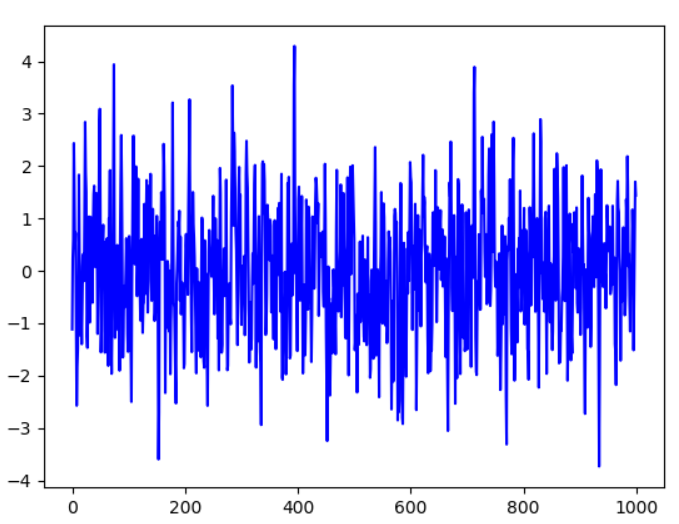
\includegraphics[height=5cm]{images/f000013}
\end{figure}
无论是ARMA还是ARIMA拟合,我们都可以得到较为正确的数据,同时残差的ACF和PACF也表明其是白噪声序列,运行结果如下所示:
\begin{figure}[H]
	\caption{程序运行结果}
	\label{f000014}
	\centering
	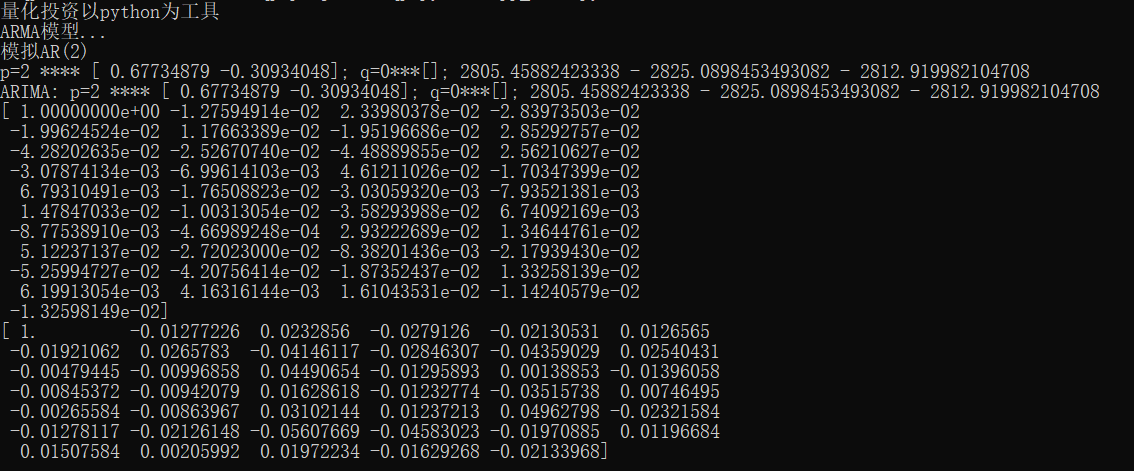
\includegraphics[height=5cm]{images/f000014}
\end{figure}
残差的自相关系数函数ACF图:
\begin{figure}[H]
	\caption{残差的自相关系数函数ACF图}
	\label{f000015}
	\centering
	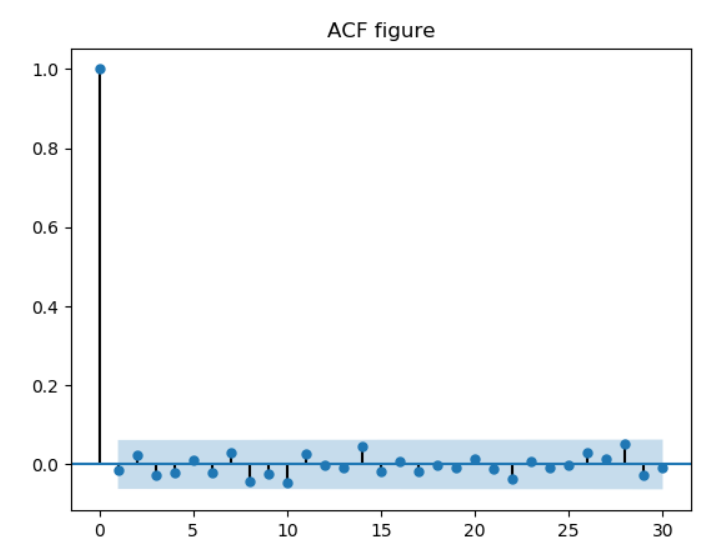
\includegraphics[height=5cm]{images/f000015}
\end{figure}
残差的偏自相关系数函数PACF图:
\begin{figure}[H]
	\caption{残差的偏自相关系数函数PACF图}
	\label{f000016}
	\centering
	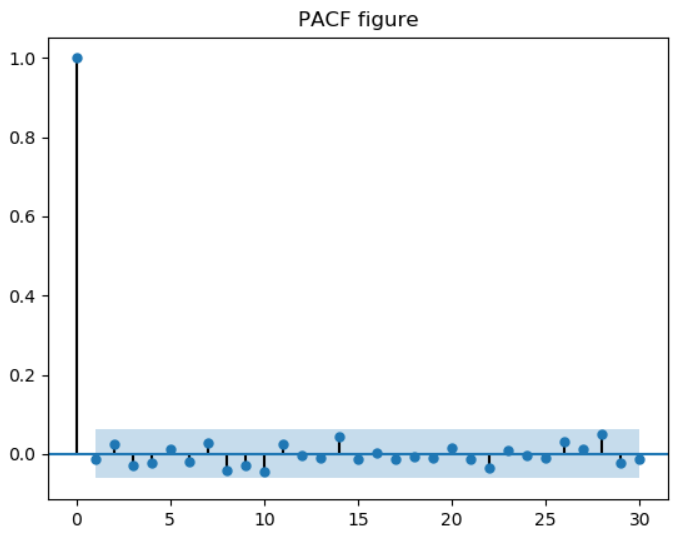
\includegraphics[height=5cm]{images/f000016}
\end{figure}
由ACF和PACF图可以看出,我们残差是比较典型的随机白噪声序列,由此可见我们拟合还是很好的。
\subsubsection{展望}
在理解了基本理论之后,我们将引入最终的ARIMA模型,并用ARIMA模型来拟合真实上证综指收盘价时间序列,并用我们的拟合模型来预测最后5日的收盘价,在这个实际例子中,看我们模型的表现如何。
\subsection{ARIMA模型}
\subsubsection{背景}
我们不仅可以对当前时间点数值对之前时间点数值进行建模,我们也可以对前面时间点随机噪声对当前时间点的影响进行建模,同时由于原始信号可能非常不平稳,但是我们求出其差值序列后,可能就变为平稳序列了,这就是ARIMA模型要解决的问题。为了讨论ARIMA模型,我们首先介绍差分的概念:
\begin{equation}
\begin{aligned}
\{ x_1,x_2,...,x_N \} \\
\{d_1^{1},d_2^{1},...,d_{N-1}^{1}\}=\{x_2-x_1,x_3-x_2,...,x_{N}-x_{N-1}\} \\
\{d_1^{2},d_2^{2},...,d_{N-1}^{2}\}=\{d_2^{1}-d_1^{1},d_3^{1}-d_2^{1},...,d_{N-1}^{1}-d_{N-1}^{1}\}
\end{aligned}
\label{e000030}
\end{equation}
上式中分别为原始时序信号,然后是一阶差分和二阶差分。
\subsubsection{模型选择标准}
\paragraph{BIC定义}
我们已经介绍过一个模型选择标准AIC(Akaike Information Criterion),其会惩罚参数多的模型,因为这些模型容易产生过拟合(Overfitting)。接下来我们要介绍另一个模型选择参数BIC(Bayes Information Criterion),与AIC相比,其会更倾向于惩罚参数多的模型,同样是值越小越好,BIC定义如下所示:
\begin{equation}
BIC=-2\log (L) + k \log N
\label{e000031}
\end{equation}
其中L为似然函数的最大值,k为模型的参数,N为数据点个数。
\paragraph{Ljung-Box检测}
我们的缺省假设$H_{0}$为:对于一个拟合的时序信号,对所有滞后时点lags,都是独立同分布(i.i.d)的,即不存在相关性。\newline
备择假设$H_{a}$为:这些信号不是独立同分布(i.i.d)的,具有相关性。\newline
我们定义统计量Q:
\begin{equation}
Q=n(n+2)\sum_{k=1}^{h} \frac{\hat{\rho}_{k}^{2}}{n-k}
\label{e000032}
\end{equation}
式\ref{e000032}中$n$为时间序列长度,$h$为最大滞后期数,$\rho _{k}$第$k$自相关系数。Ljung-Box检测原理比较复杂,但是在python语言中,经过运算可以求出Q值,以及大于Q值的概率,实际上我们看1$\sim$12滞后期的Q值和大于Q值的概率,如果该概率小于显著水平如0.05时,就拒绝缺省假设(不存在相关性),选择备择假设,否则反之。
\subsubsection{定义}
同时考虑之前时间点的信号和噪声值,我们就可以得到如下ARMA模型:
\begin{equation}
x_{t}=\alpha _{1}x_{t-1} + \alpha _{2}x_{t-2} + ... + \alpha _{p}x_{t-p} + w_{t} + \beta _1w_{t-1} + \beta _2w_{t-2}+...+ + \beta _{q}w_{t-q}
\label{e000033}
\end{equation}
如果我们对欲研究的信号求出一阶或二阶差分,然后再利用式\ref{e000033}的模型,就是ARIMA模型了。其中$\{ w_{t} \}$为白噪声,其均值为0,方差为$\sigma ^{2}$。\newline
其特性方程可以表示为:
\begin{equation}
\theta _{p}(B)x_{t}=\phi _{q}(B)w_{t}
\label{e000034}
\end{equation}
由上面的讨论可以看出,AR(p)和MA(q)都是ARIMA模型的特殊情况,在同样精度的条件下,ARIMA模型所需参数最小。
\subsubsection{数据仿真}
在理解了ARIMA模型定义之后,我们来模拟一下ARIMA过程。假设我们要模拟的ARIMA模型为:
\begin{equation}
\begin{aligned}
x_{t}=\alpha _{1}x_{t-1} + \alpha _{2}x_{t-2} + w_{t} + \beta _1w_{t-1} + \beta _2w_{t-2} \\
=1.2 \times x_{t-1} - 0.7 \times x_{t-2} + w_{t} - 0.06 \times w_{t-1} - 0.02 \times w_{t-2}
\end{aligned}
\label{e000035}
\end{equation}
生成模拟数据并利用ARIMA拟合的程序如下所示:
\lstset{language=PYTHON, caption={AR数据模拟和拟合示例}, label={c000005}}
\begin{lstlisting}
    def simulate_arima_p_d_q(self):
        print('模拟ARIMA(p,d,q)过程')
        np.random.seed(8)
        alpha1 = 1.2
        alpha2 = -0.7
        beta1 = -0.06
        beta2 = -0.02
        w = np.random.standard_normal(size=1000)
        x = w
        for t in range(2, len(w)):
            x[t] = alpha1 * x[t-1] + alpha2*x[t-2] + w[t] + beta1 * w[t-1] + beta2*w[t-2]
        plt.plot(x, c='b')
        plt.title('ARIMA(p, d, q) Figure')
        plt.show()
        # 查看ACF
        acfs = stattools.acf(x)
        print('ARIMA(q,d,q) ACFS:\r\n{0}'.format(acfs))
        tsaplots.plot_acf(x, use_vlines=True, lags=30)
        plt.title('ARIMA(p,d,q) ACF')
        plt.show()
        # ARIMA拟合
        min_ABQIC = sys.float_info.max
        arima_model = None
        break_loop = False
        '''
        for p in range(0, 5):
            if break_loop:
                break
            for q in range(0, 5):
                print('try {0}, d, {1}...'.format(p, q))
                try:
                    arima_p_d_q = ARIMA(x, order=(p, 0, q)).fit(disp=False)
                    print('..... fit ok')
                    if arima_p_d_q.aic < min_ABQIC:
                        print('..... record good model')
                        min_ABQIC = arima_p_d_q.aic
                        arima_model = arima_p_d_q
                        #if 1==p and 1==q:
                        #    break_loop = True
                except Exception as ex:
                    print('.....!!!!!! Exception')
        print('ARIMA: p={0} **** {1}; q={2}***{3}; {4} - {5} - {6}'. \
                    format(arima_model.k_ar, arima_model.arparams, 
                    arima_model.k_ma, arima_model.maparams, 
                    arima_model.aic, arima_model.bic, 
                    arima_model.hqic)
        )
        '''
        arima_model = ARIMA(x, order=(2, 0, 2)).fit(disp=False)
        print('God_View:ARIMA: p={0} **** {1}; q={2}***{3}; {4} - {5} - {6}'. \
                    format(arima_model.k_ar, arima_model.arparams, 
                    arima_model.k_ma, arima_model.maparams, 
                    arima_model.aic, arima_model.bic, 
                    arima_model.hqic)
        )
        resid = arima_model.resid
        # 绘制ACF
        acfs = stattools.acf(resid)
        print(acfs)
        tsaplots.plot_acf(resid, use_vlines=True, lags=30)
        plt.title('ARIMA(p,d,q) ACF figure')
        plt.show()
        pacfs = stattools.pacf(resid)
        print(pacfs)
        tsaplots.plot_pacf(resid, use_vlines=True, lags=30)
        plt.title('ARIMA(p,d,q) PACF figure')
        plt.show()
\end{lstlisting}
生成的时序信号x为:
\begin{figure}[H]
	\caption{原始模拟信号图}
	\label{f000017}
	\centering
	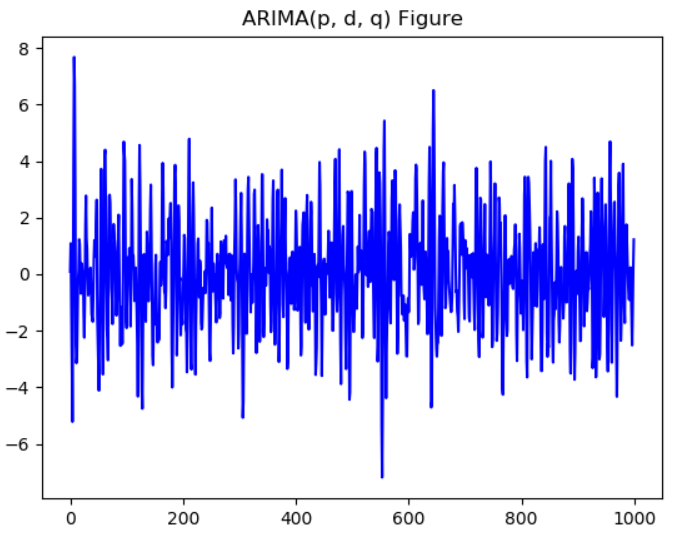
\includegraphics[height=5cm]{images/f000017}
\end{figure}
该信号的自相关系数函数ACF图为:
\begin{figure}[H]
	\caption{原始模拟信号ACF图}
	\label{f000018}
	\centering
	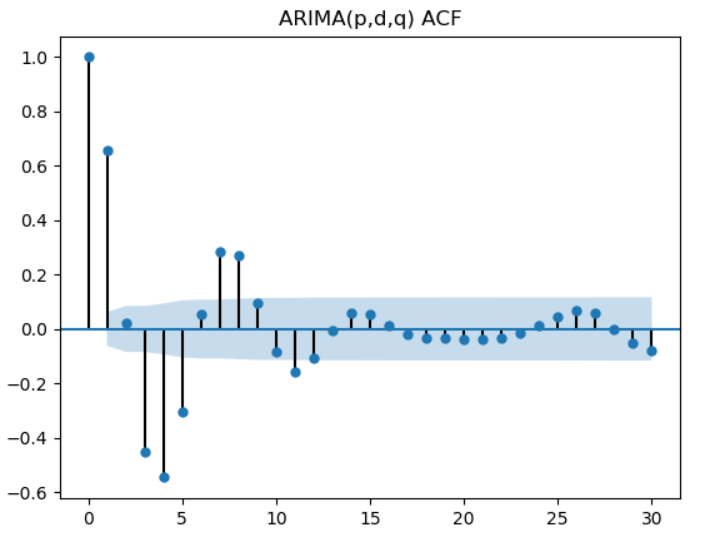
\includegraphics[height=5cm]{images/f000018}
\end{figure}
由图中可以看出,该信号具有非常强的自相关性。\newline
接着我们用ARIMA模型来模拟该信号,上面程序注释部分为求最佳ARIMA模型的p和q参数,以AIC作为模型选择标准,因为我们知道模型为ARIMA(2,0,2),所以我们同时也用ARIMA(2,0,2)来进行拟合,程序运行结果如下所示:
\begin{figure}[H]
	\caption{程序运行结果}
	\label{f000019}
	\centering
	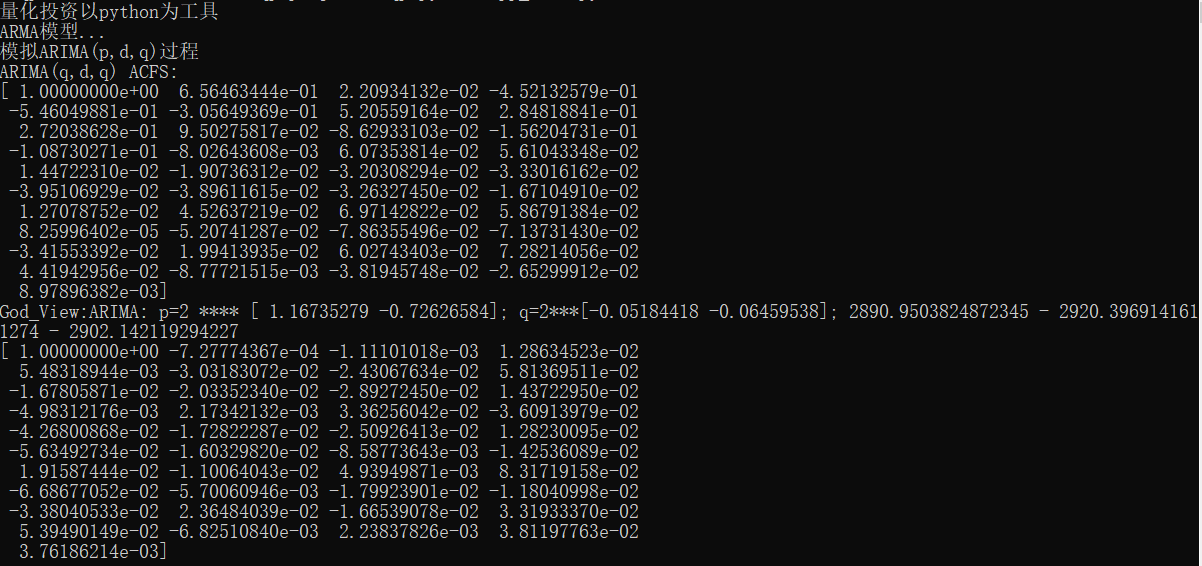
\includegraphics[height=5cm]{images/f000019}
\end{figure}
接着我们求出残差序列,残差序列自相关系数函数ACF图如下所示:
\begin{figure}[H]
	\caption{残差自相关系数函数ACF图}
	\label{f000020}
	\centering
	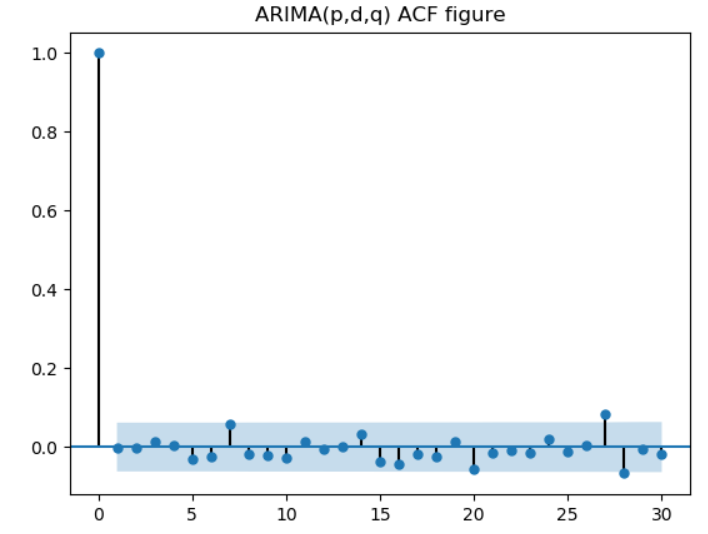
\includegraphics[height=5cm]{images/f000020}
\end{figure}
残差序列偏自相关系数函数图PACF如下所示:
\begin{figure}[H]
	\caption{残差偏自相关系数函数ACF图}
	\label{f000021}
	\centering
	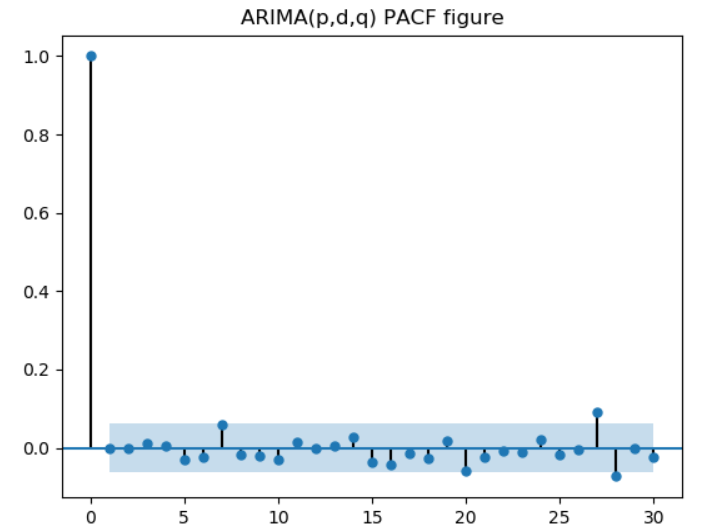
\includegraphics[height=5cm]{images/f000021}
\end{figure}
由图中可以看出,残差序列基本上是白噪声信号。
\subsubsection{金融数据拟合及预测}
接下来我们用ARIMA模型,来拟合上证综指收盘价,我们利用除最后3天的数据来得出ARIMA模型,然后利用拟合出的ARIMA模型来预测后3天的收盘价,来看我们模型的性能。根据经验,对于股票的收盘数据来说,采用取对数后再求1阶差分的形式,可以取得更好的效果,因此我们会先对数据进行预处理,然后再来用ARIMA模型来拟合数据。\newline
程序如下所示:
\lstset{language=PYTHON, caption={ARIMA数据拟合上证综指收盘价}, label={c000007}}
\begin{lstlisting}
    def arima_demo(self):
        register_matplotlib_converters()
        data = pd.read_csv(self.data_file, sep='\t', index_col='Trddt')
        sh_index = data[data.Indexcd==1]
        sh_index.index = pd.to_datetime(sh_index.index)
        raw_data = sh_index.Clsindex
        train_data = raw_data[:-3]
        close_price = np.log(train_data)
        plt.plot(close_price)
        plt.show()
        print(train_data.head(n=3))
        # ARIMA拟合
        min_ABQIC = sys.float_info.max
        arima_model = None
        for p in range(0, 5):
            for q in range(0, 5):
                print('try {0}, d, {1}...'.format(p, q))
                try:
                    arima_p_d_q = ARIMA(close_price, order=(p, 1, q)).fit(disp=False)
                    print('..... fit ok')
                    if arima_p_d_q.aic < min_ABQIC:
                        print('..... record good model')
                        min_ABQIC = arima_p_d_q.aic
                        arima_model = arima_p_d_q
                except Exception as ex:
                    print('.....!!!!!! {0}'.format(ex))
        print('ARIMA: p={0} **** {1}; q={2}***{3}; {4} - {5} - {6}'. \
                    format(arima_model.k_ar, arima_model.arparams, 
                    arima_model.k_ma, arima_model.maparams, 
                    arima_model.aic, arima_model.bic, 
                    arima_model.hqic)
        )
        resid = arima_model.resid
        # 绘制ACF
        acfs = stattools.acf(resid)
        print(acfs)
        tsaplots.plot_acf(resid, use_vlines=True, lags=30)
        plt.title('ARIMA(p,d,q) ACF figure')
        plt.show()
        pacfs = stattools.pacf(resid)
        print(pacfs)
        tsaplots.plot_pacf(resid, use_vlines=True, lags=30)
        plt.title('ARIMA(p,d,q) PACF figure')
        plt.show()
        # ADF检验
        resid_adf = unitroot.ADF(resid)
        print('stat={0:0.4f} vs 1%_cv={1:0.4f}'.format(resid_adf.stat, resid_adf.critical_values['1%']))
        if resid_adf.stat < resid_adf.critical_values['1%']:
            print('resid为稳定时间序列 ^_^')
        else:
            print('resid为非稳定时间序列!!!!!')
        # Ljung-Box检验
        resid_ljung_box = stattools.q_stat(stattools.acf(resid)[1:12], len(resid))
        resid_lbv = resid_ljung_box[1][-1]
        print('resid_ljung_box_value={0}'.format(resid_lbv))
        # 0.05为显著性水平
        if resid_lbv < 0.05:
            print('resid为平稳时间序列 ^_^')
        else:
            print('resid为非平稳时间序列!!!!!!!')
        # 预测
        y = arima_model.forecast(3)[0] #(len(train_data), len(raw_data), dynamic=True)
        print('预测值:{0}'.format(np.exp(y)))
        print('row_data:{0}'.format(raw_data))
        print('train_data:{0}'.format(train_data))
\end{lstlisting}
我们首先绘制出上证综指收盘价曲线:
\begin{figure}[H]
	\caption{上证综指收盘价}
	\label{f000023}
	\centering
	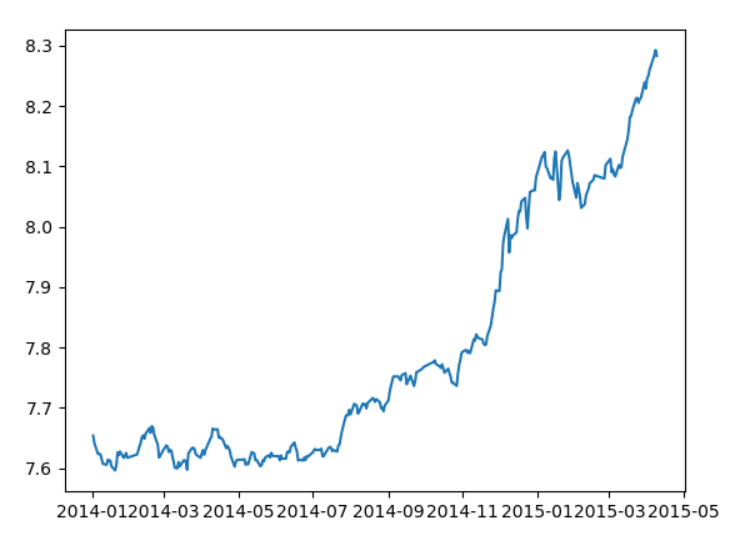
\includegraphics[height=5cm]{images/f000023}
\end{figure}
接着我们对该数据经过对数差分后,利用ARIMA来进行拟合,得到拟合模型为:
\begin{figure}[H]
	\caption{拟合后的ARIMA模型}
	\label{f000024}
	\centering
	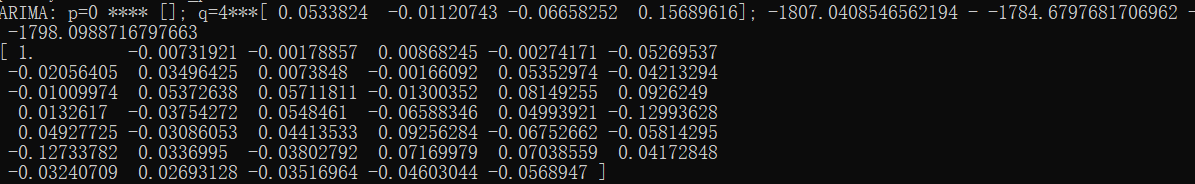
\includegraphics[height=2cm]{images/f000024}
\end{figure}
残差序列的自相关系数函数ACF图为:
\begin{figure}[H]
	\caption{残差序列的自相关系数函数ACF图}
	\label{f000025}
	\centering
	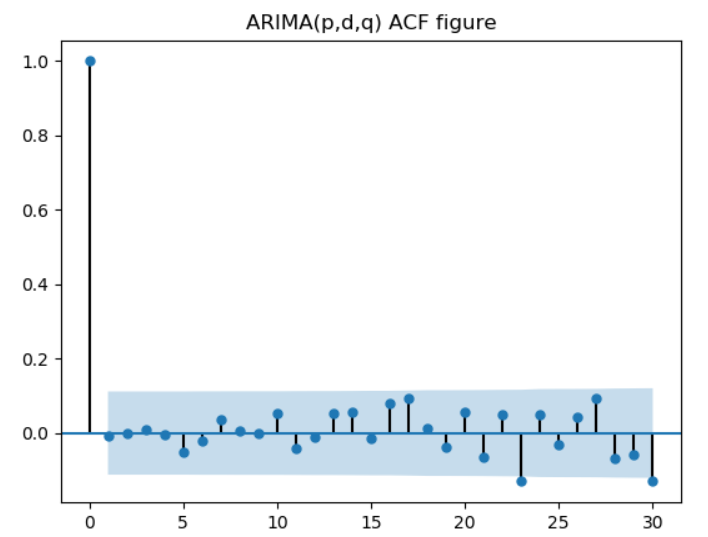
\includegraphics[height=5cm]{images/f000025}
\end{figure}
残差序列的偏自相关系数函数PACF图为:
\begin{figure}[H]
	\caption{残差序列的偏自相关系数函数PACF图}
	\label{f000026}
	\centering
	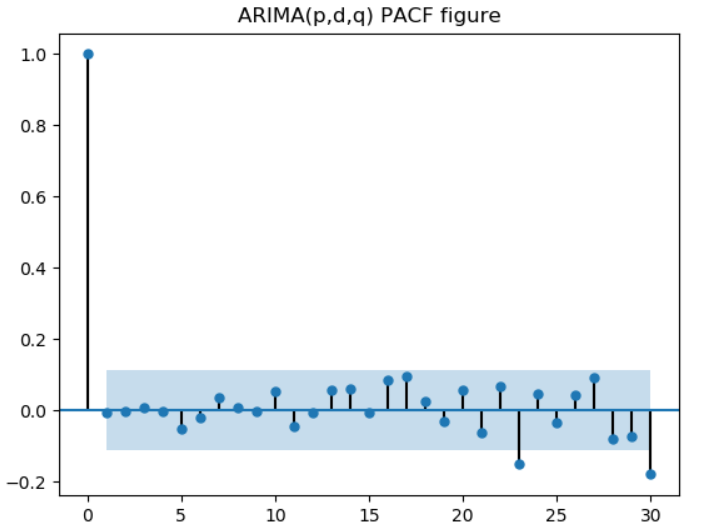
\includegraphics[height=5cm]{images/f000026}
\end{figure}
进行ADF检验的结果为:
\begin{figure}[H]
	\caption{ADF检验的结果}
	\label{f000027}
	\centering
	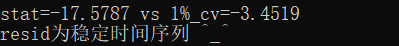
\includegraphics[height=1cm]{images/f000027}
\end{figure}
进行Ljung-Box检验结果为:
\begin{figure}[H]
	\caption{Ljung-Box检验结果}
	\label{f000028}
	\centering
	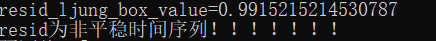
\includegraphics[height=1cm]{images/f000028}
\end{figure}
最后我们拿我们的模型进行预测,后三天的预测结果为:
\begin{figure}[H]
	\caption{ARIMA模型预测后三天结果}
	\label{f000029}
	\centering
	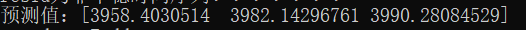
\includegraphics[height=0.6cm]{images/f000029}
\end{figure}
实际值为:
\begin{figure}[H]
	\caption{实际收盘价}
	\label{f000030}
	\centering
	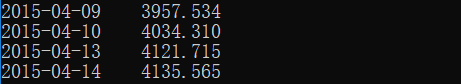
\includegraphics[height=2cm]{images/f000030}
\end{figure}
我们看到,我们的模型基本预测出了后三天的连涨行情,只不过上涨的幅度有一些小。

\maketitle\begin{center}
\Large \textbf{第3章 GARCH模型}
\end{center}
\begin{abstract}
在本章中我们将首先讲述条件异方差模型GARCH(Generalized AutoRegressive Conditional Heteroskedastic),
并将GARCH模型用于实际金融时间序列数据拟合。aqt002.py
\end{abstract}
\section{GARCH模型}





python的ARIMA:   https://www.colabug.com/3933896.html
Ln125 Advanced Algorithmic Trading


\section{汇总}
f000022
c000008
e000050





















\maketitle\begin{center}
\Large \textbf{第4章 协整模型}
\end{center}
\begin{abstract}
在本章中我们将首先讲述条件异方差模型GARCH(Generalized AutoRegressive Conditional Heteroskedastic),
并将GARCH模型用于实际金融时间序列数据拟合。aqt002.py
\end{abstract}
\section{协整模型}

\maketitle\begin{center}
\Large \textbf{第5章 卡尔曼滤波}
\end{center}
\begin{abstract}
在本章中我们将首先讲述条件异方差模型GARCH(Generalized AutoRegressive Conditional Heteroskedastic),
并将GARCH模型用于实际金融时间序列数据拟合。aqt002.py
\end{abstract}
\section{卡尔曼滤波}

\maketitle\begin{center}
\Large \textbf{第6章 隐马可夫模型}
\end{center}
\begin{abstract}
在本章中我们将首先讲述条件异方差模型GARCH(Generalized AutoRegressive Conditional Heteroskedastic),
并将GARCH模型用于实际金融时间序列数据拟合。aqt002.py
\end{abstract}
\section{隐马可夫模型}

\maketitle\begin{center}
\Large \textbf{第7章 统计套利策略}
\end{center}
\begin{abstract}
在本章中我们将首先讲述条件异方差模型GARCH(Generalized AutoRegressive Conditional Heteroskedastic),
并将GARCH模型用于实际金融时间序列数据拟合。aqt002.py
\end{abstract}
\section{统计套利策略}

\maketitle\begin{center}
\Large \textbf{第8章 机器学习}
\end{center}
\begin{abstract}
在本章中我们将首先讲述条件异方差模型GARCH(Generalized AutoRegressive Conditional Heteroskedastic),
并将GARCH模型用于实际金融时间序列数据拟合。aqt002.py
\end{abstract}
\section{机器学习}

\maketitle\begin{center}
\Large \textbf{第9章 高频交易}
\end{center}
\begin{abstract}
在本章中我们将首先讲述条件异方差模型GARCH(Generalized AutoRegressive Conditional Heteroskedastic),
并将GARCH模型用于实际金融时间序列数据拟合。aqt002.py
\end{abstract}
\section{高频日内交易}

\maketitle\begin{center}
\Large \textbf{第10章 程序化CTA}
\end{center}
\begin{abstract}
在本章中我们将首先讲述条件异方差模型GARCH(Generalized AutoRegressive Conditional Heteroskedastic),
并将GARCH模型用于实际金融时间序列数据拟合。aqt002.py
\end{abstract}
\section{程序化CTA}



参考文献:
\cite{ex1}---\cite{ex2}---\cite{refa001}

\newpage

\bibliographystyle{plainnat}
\bibliography{nips}

\appendix


\end{document}
